\section{Experiments}

We evaluate our approach in the Safety Gymnasium \cite{ji2023safety} environment, focusing on the \texttt{PointGoal} task under different cost limits.
Safety Gymnasium provides two cost definitions, a binary indicator and object-specific values, and the object-specific cost (\texttt{constrain\_indicator=False}) is adopted in all experiments.
The proposed approach is evaluated in terms of constraint satisfaction performance by comparing it with CPO \cite{achiam2017constrained}, PPO Lagrangian \cite{ray2019benchmarking}, IPO \cite{liu2020ipo}, and CPPO \cite{stooke2020responsive}, using the implementations provided by Omnisafe \cite{ji2024omnisafe}.

\subsection{Results}

Figures~\ref{fig:point_goal_results_vertical1} and \ref{fig:point_goal_results_vertical2} present the results under different cost limits.
Each figure shows how return, cost return, and the Lagrange multiplier evolve during training, highlighting how varying cost limits affect the agent's performance and constraint satisfaction.
Since all methods except ours define the constraint in terms of cumulative cost, the threshold for our method was set to 1/1000 of theirs (as each episode consists of 1,000 steps).
From Fig.~\ref{fig:point_goal_results_vertical1} (e) and Fig.~\ref{fig:point_goal_results_vertical2} (b), (e), it can be observed that our proposed method consistently satisfies the constraints across different settings, unlike the other methods.
%%% 수정 필요
When the constraint is enforced too strictly to be satisfied, as in Fig.~\ref{fig:point_goal_results_vertical1} (b), \textcolor{red}{none of the methods can fully satisfy it, but our proposed method and CPO come closest to meeting the constraint, achieving much lower cost returns than the others.}
In particular, as shown in Fig.~\ref{fig:point_goal_results_vertical1} (a) and (b), our method achieves a similar level of constraint satisfaction as CPO, while obtaining \textcolor{red}{approximately 1.8 times higher} return performance.  % 2배 언급 수정
%%%
However, Fig.~\ref{fig:point_goal_results_vertical1} (d) suggests that the reward performance can be lower than that of some of the other methods.
This is due to the use of state-wise cost constraints in our method, unlike the compared approaches that enforce constraints defined on cumulative cost return, which leads the policy to converge in a more local and conservative manner.
As a result, the constraints are well satisfied, but the reward performance can converge to a lower level.
% This is a common trade-off in constrained RL.
In addition, as shown in Fig.~\ref{fig:point_goal_results_vertical1} (f) and Fig.~\ref{fig:point_goal_results_vertical2} (c) and (f), when comparing the values of the Lagrange multiplier, our proposed method satisfies the constraints, resulting in bounded values or decreasing trends.
An exception occurs when the cost limit is set to 0.5, which is particularly strict and difficult to satisfy, leading to continuously increasing values.

\begin{figure}[H]
    \centering

    % ----- 공통 범례 -----
    \begin{subfigure}{1.0\textwidth}
        \centering
        
\includegraphics[width=\linewidth]{figure/PointGoal/limit 1/legend_common.pdf}
    \end{subfigure}

    \vspace{0.5em} % 범례와 밑 그림 사이 간격 조정

    % ----- Limit 0.5 (왼쪽 열) -----
    \begin{minipage}{0.48\textwidth}
        \centering
        \begin{subfigure}{\linewidth}
            \centering
            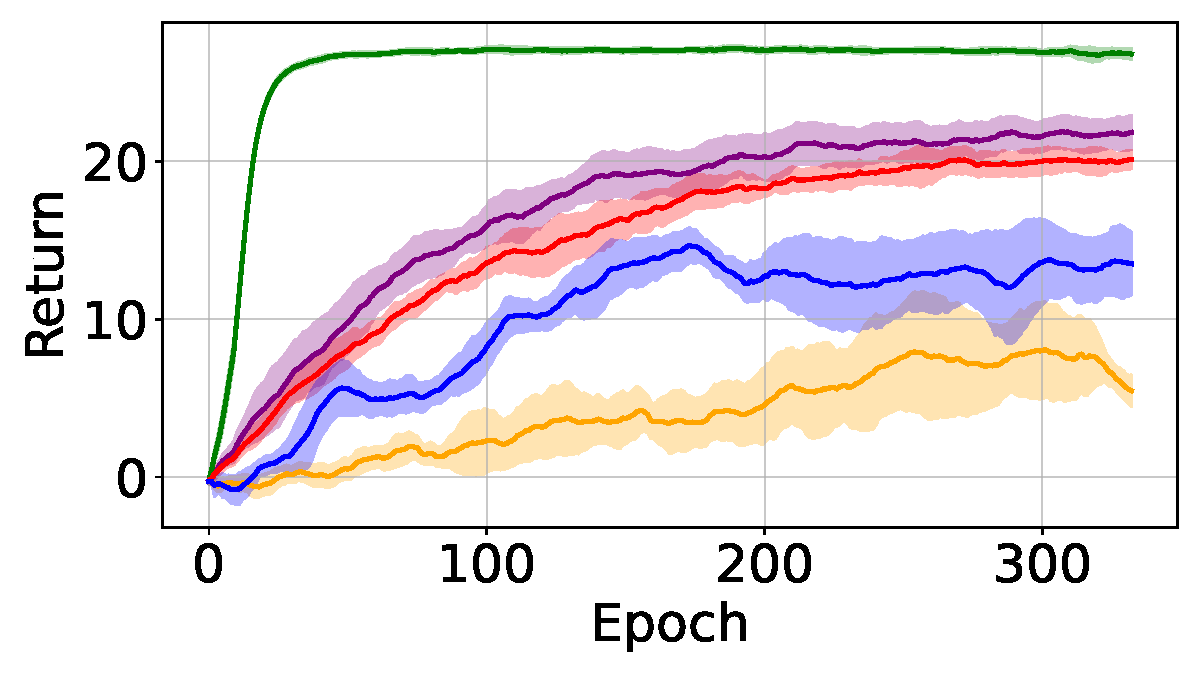
\includegraphics[width=\linewidth]{figure/PointGoal/limit 0.5/EpRet.pdf}
            \caption{Return over epochs}
        \end{subfigure}

        \begin{subfigure}{\linewidth}
            \centering
            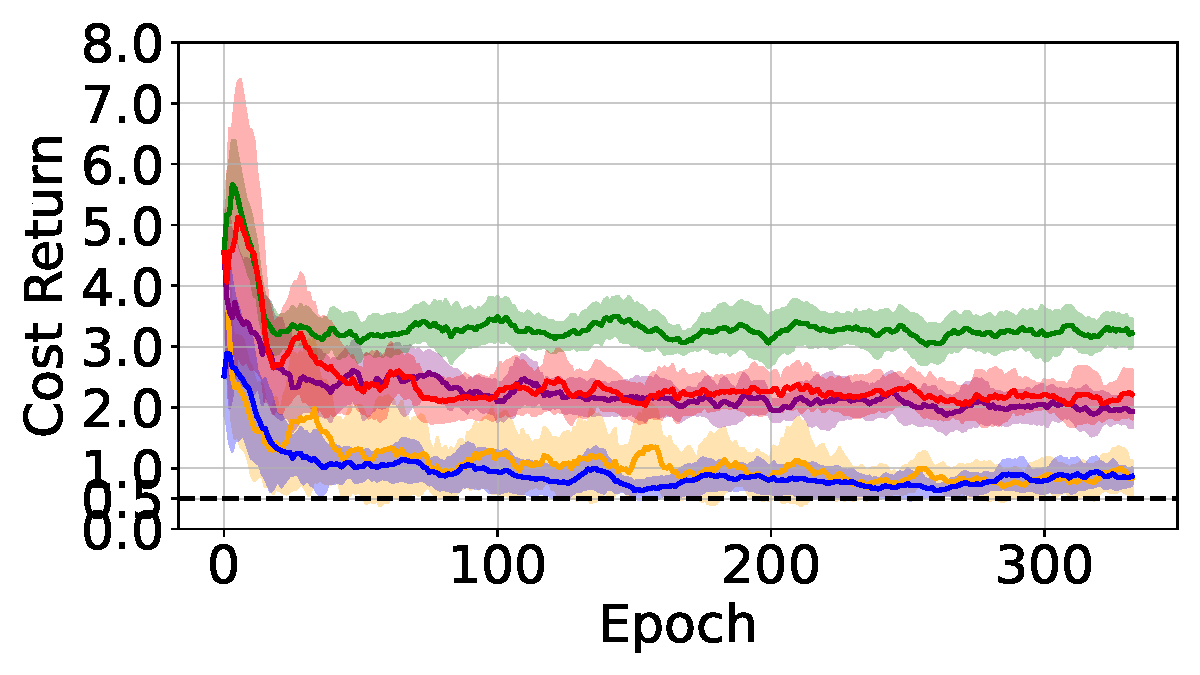
\includegraphics[width=\linewidth]{figure/PointGoal/limit 0.5/EpCost.pdf}
            \caption{Cost Return over epochs}
        \end{subfigure}

        \begin{subfigure}{\linewidth}
            \centering
            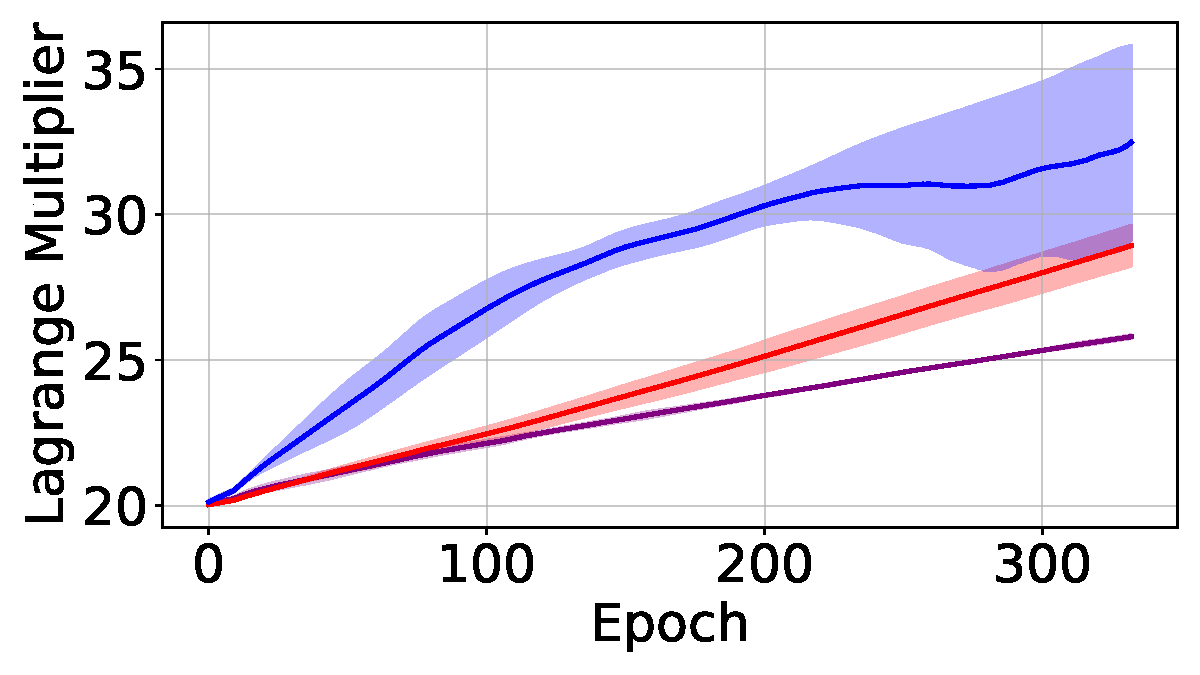
\includegraphics[width=\linewidth]{figure/PointGoal/limit 0.5/lagrange.pdf}
            \caption{Lagrange multipliers over epochs}
        \end{subfigure}

        \caption*{Cost return limit: 0.5}
    \end{minipage}
    \hfill
    % ----- Limit 1 (오른쪽 열) -----
    \begin{minipage}{0.48\textwidth}
        \centering
        \begin{subfigure}{\linewidth}
            \centering
            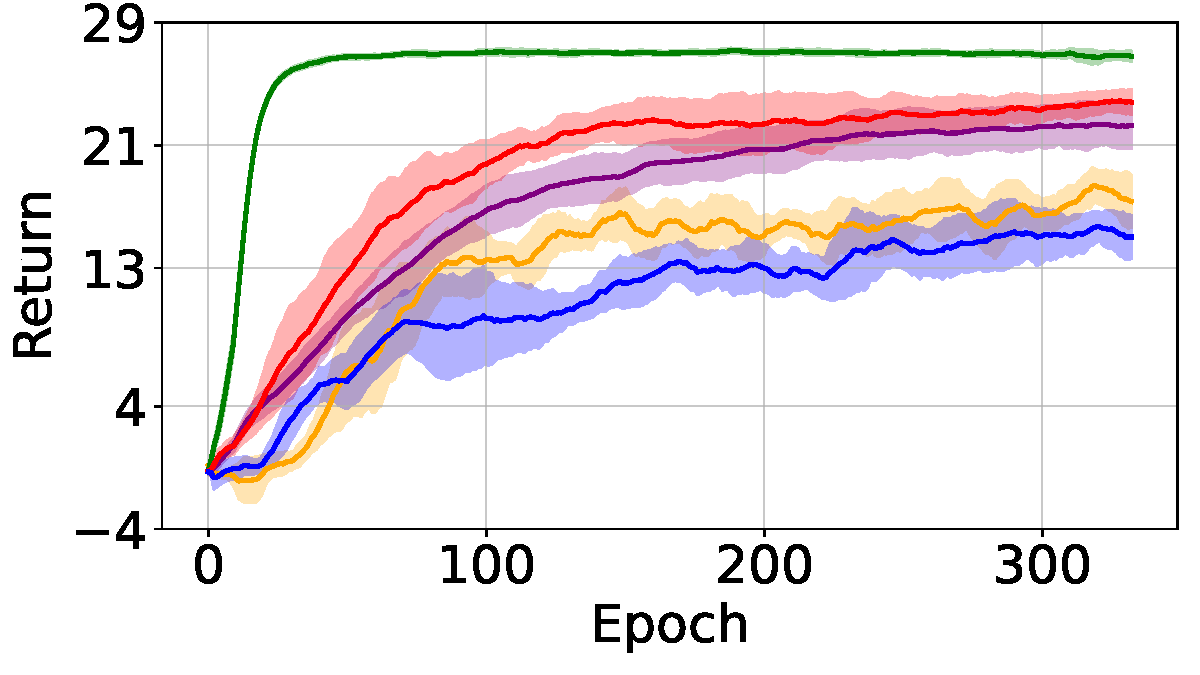
\includegraphics[width=\linewidth]{figure/PointGoal/limit 1/EpRet.pdf}
            \caption{Return over epochs}
        \end{subfigure}

        \begin{subfigure}{\linewidth}
            \centering
            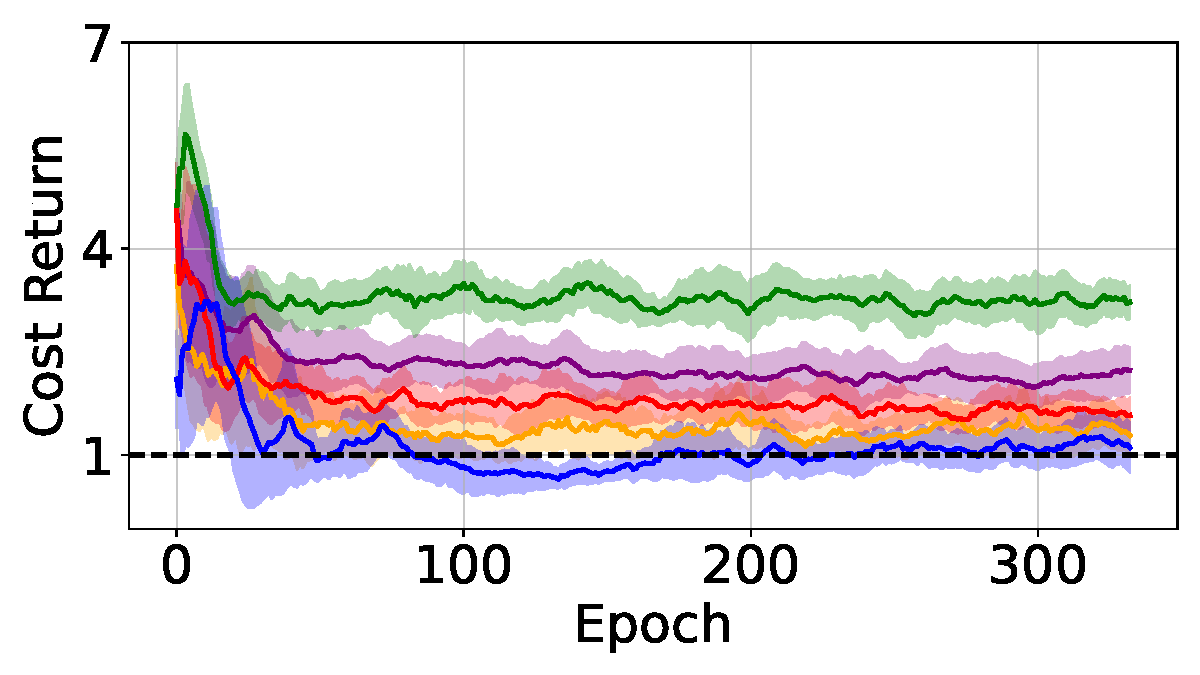
\includegraphics[width=\linewidth]{figure/PointGoal/limit 1/EpCost.pdf}
            \caption{Cost Return over epochs}
        \end{subfigure}

        \begin{subfigure}{\linewidth}
            \centering
            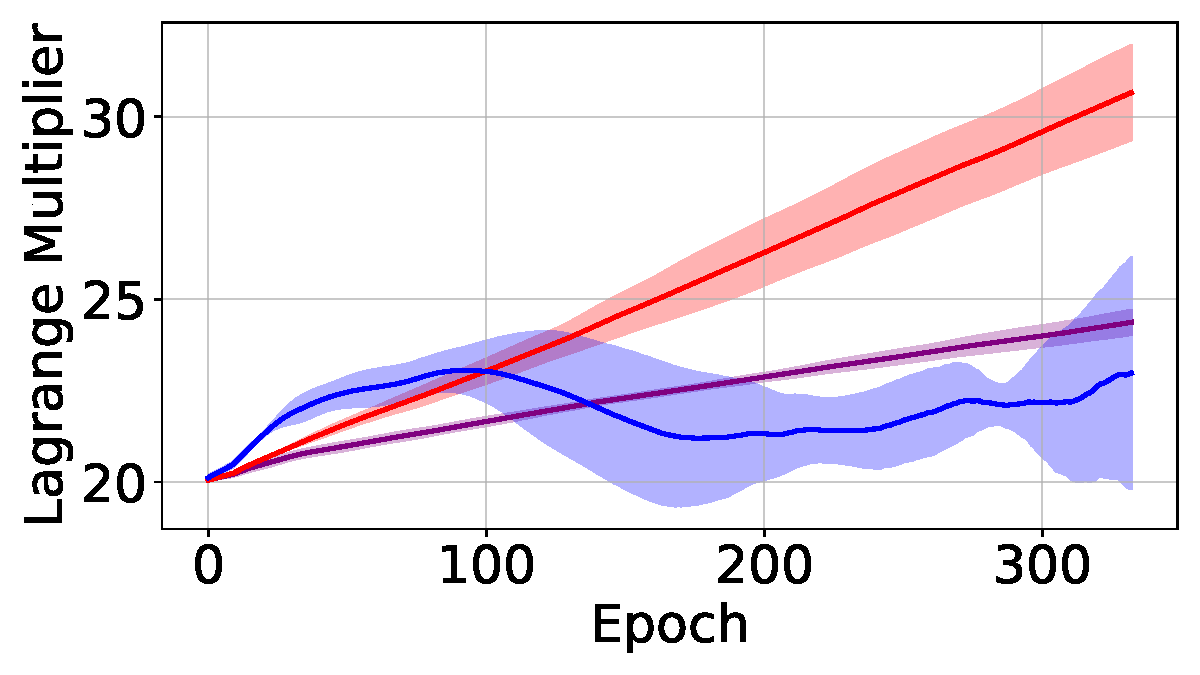
\includegraphics[width=\linewidth]{figure/PointGoal/limit 1/lagrange.pdf}
            \caption{Lagrange multipliers over epochs}
        \end{subfigure}

        \caption*{Cost return limit: 1}
    \end{minipage}

    \caption{Learning curves.
    The left column, (a)–(c), illustrates the return, cost return, and Lagrange multiplier when the cost limit is set to 0.5. 
    The right column, (d)–(f), shows the corresponding results under a cost limit of 1.0. 
    Each row presents a different metric, showing how the return (top), cost return (middle), and Lagrange multiplier (bottom) evolve over training epochs.}
    \label{fig:point_goal_results_vertical1}
\end{figure}

\begin{figure}[H]
    \centering

    % ----- 공통 범례 -----
    \begin{subfigure}{1.0\textwidth}
        \centering
        
\includegraphics[width=\linewidth]{figure/PointGoal/limit 2/legend_common.pdf}
    \end{subfigure}

    \vspace{0.5em} % 범례와 밑 그림 사이 간격 조정


    % ----- Limit 1.5 (왼쪽 열) -----
    \begin{minipage}{0.48\textwidth}
        \centering
        \begin{subfigure}{\linewidth}
            \centering
            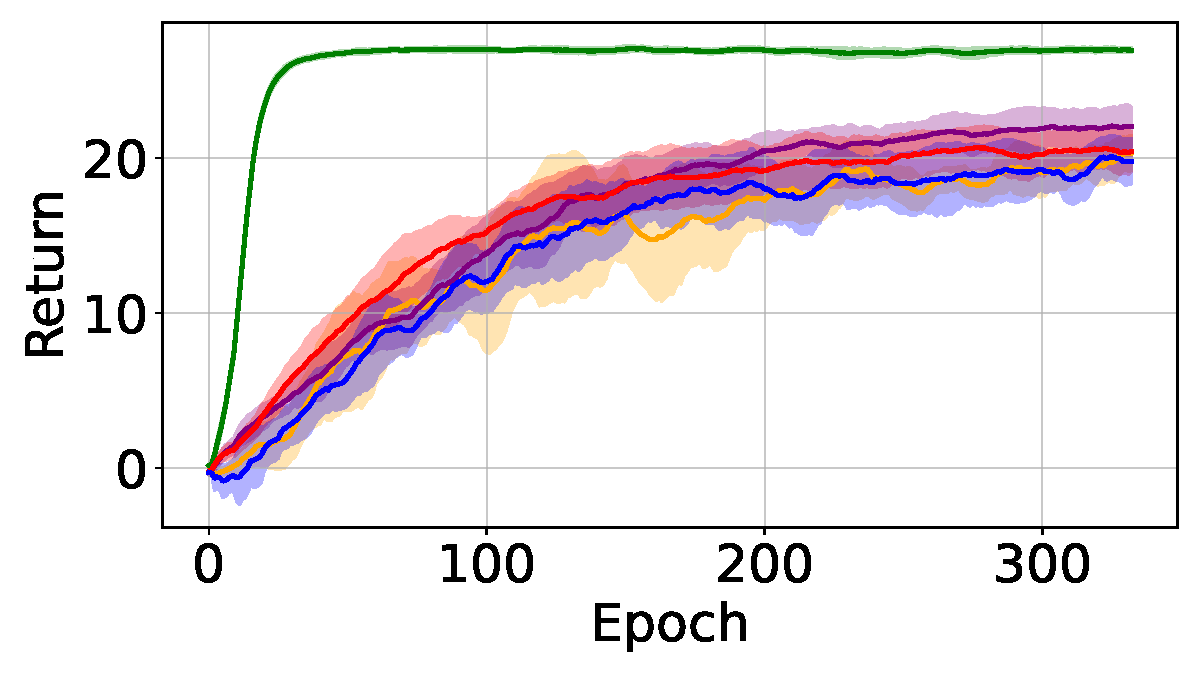
\includegraphics[width=\linewidth]{figure/PointGoal/limit 1.5/EpRet.pdf}
            \caption{Return over epochs}
        \end{subfigure}

        \begin{subfigure}{\linewidth}
            \centering
            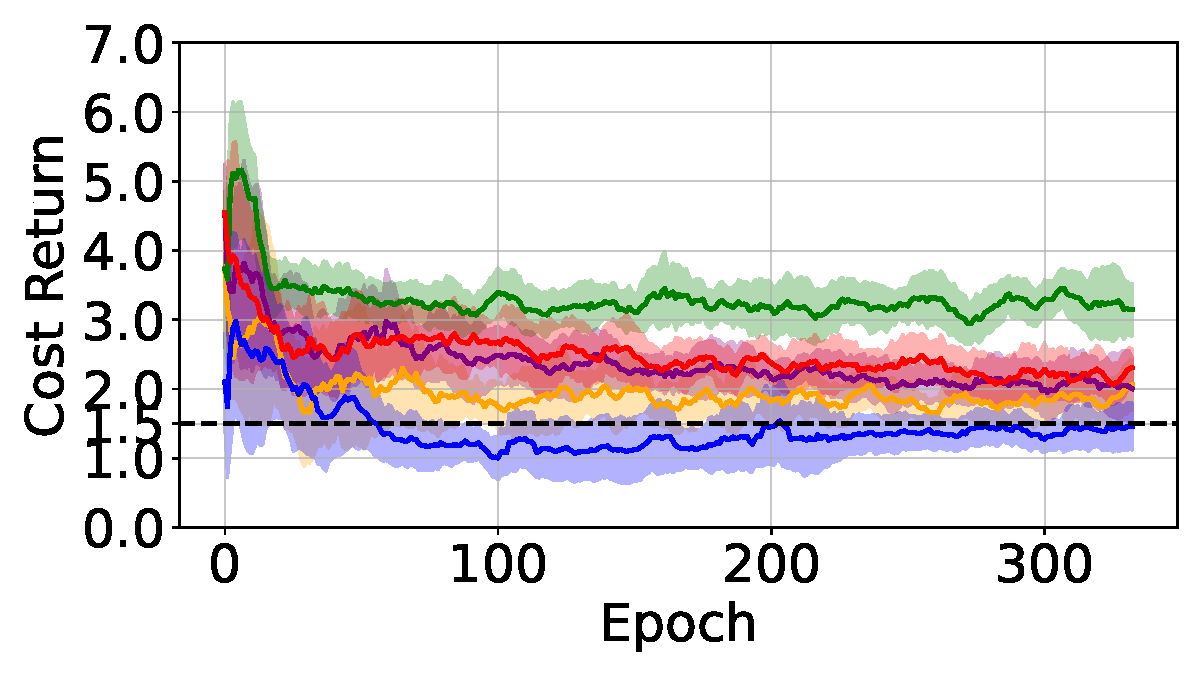
\includegraphics[width=\linewidth]{figure/PointGoal/limit 1.5/EpCost.pdf}
            \caption{Cost Return over epochs}
        \end{subfigure}

        \begin{subfigure}{\linewidth}
            \centering
            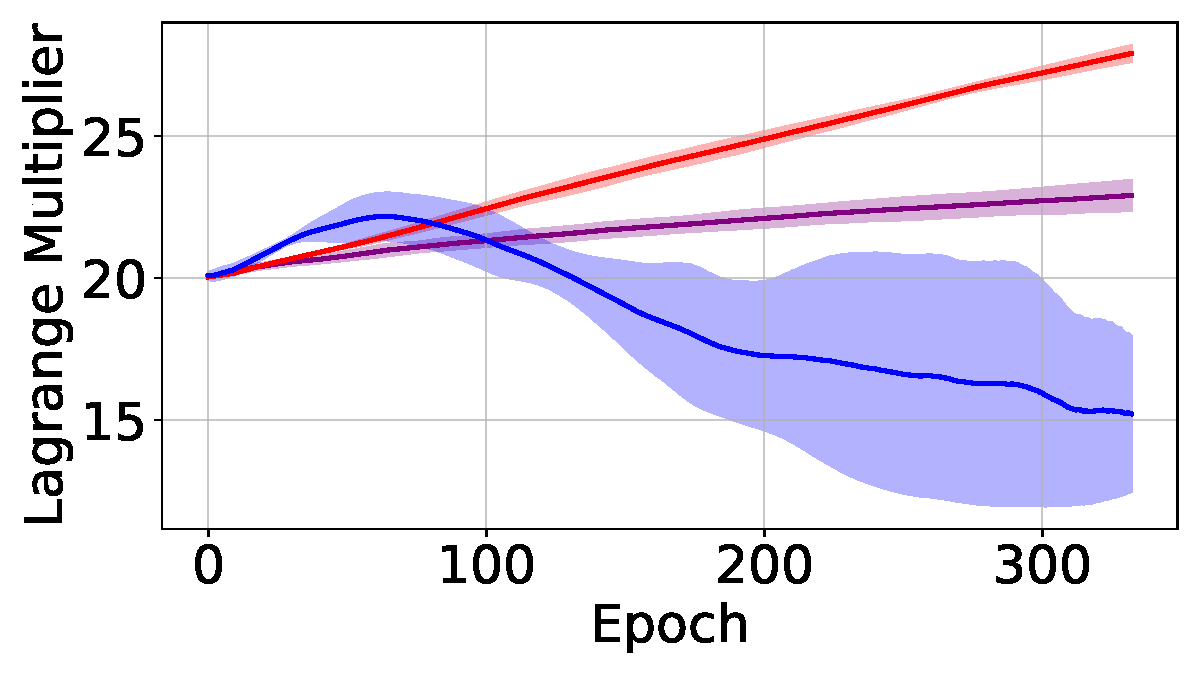
\includegraphics[width=\linewidth]{figure/PointGoal/limit 1.5/lagrange.pdf}
            \caption{Lagrange multipliers over epochs}
        \end{subfigure}

        \caption*{Cost return limit: 1.5}
    \end{minipage}
    \hfill
    % ----- Limit 2 (오른쪽 열) -----
    \begin{minipage}{0.48\textwidth}
        \centering
        \begin{subfigure}{\linewidth}
            \centering
            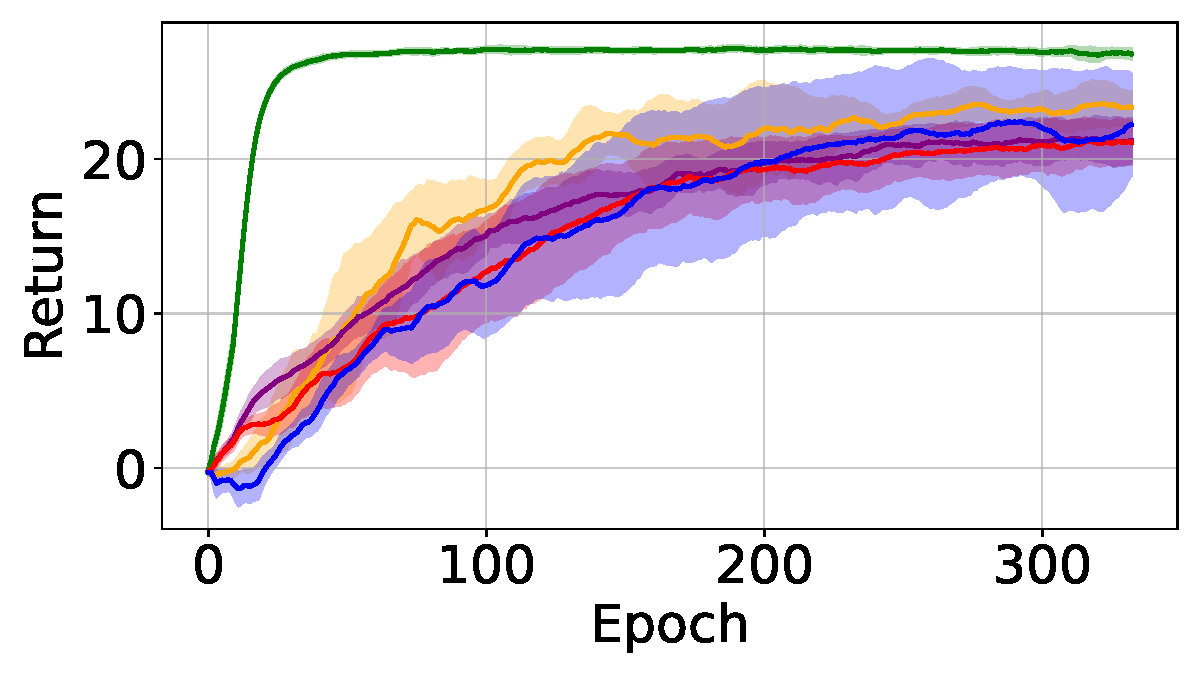
\includegraphics[width=\linewidth]{figure/PointGoal/limit 2/EpRet.pdf}
            \caption{Return over epochs}
        \end{subfigure}

        \begin{subfigure}{\linewidth}
            \centering
            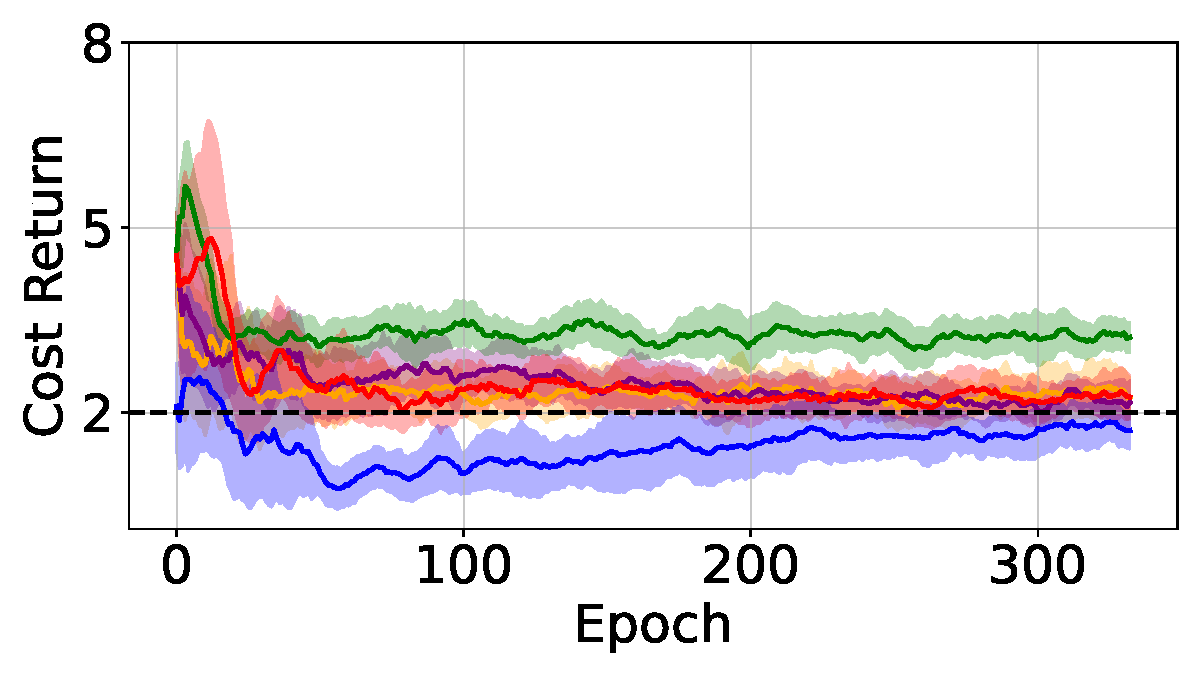
\includegraphics[width=\linewidth]{figure/PointGoal/limit 2/EpCost.pdf}
            \caption{Cost Return over epochs}
        \end{subfigure}

        \begin{subfigure}{\linewidth}
            \centering
            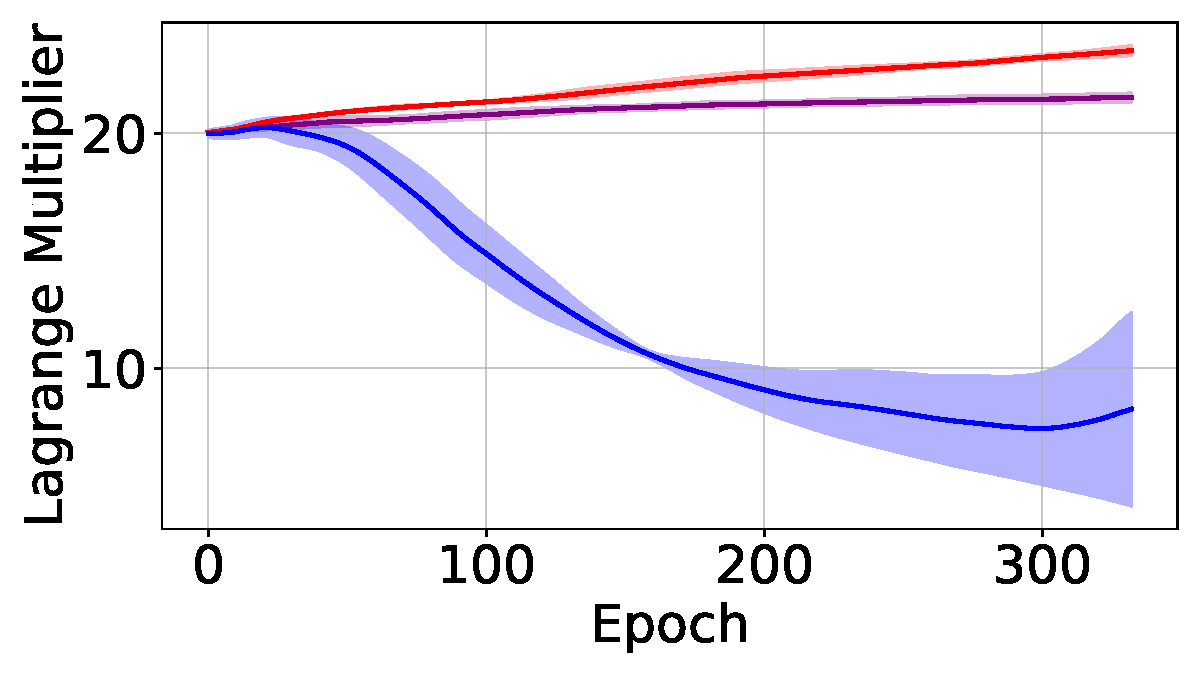
\includegraphics[width=\linewidth]{figure/PointGoal/limit 2/lagrange.pdf}
            \caption{Lagrange multipliers over epochs}
        \end{subfigure}

        \caption*{Cost return limit: 2}
    \end{minipage}

    \caption{Learning curves.
            The left column, (a)–(c), illustrates the return, cost return, and Lagrange multiplier when the cost limit is set to 1.5. 
            The right column, (d)–(f), shows the corresponding results under a cost limit of 2.0. 
            Each row presents a different metric, showing how the return (top), cost return (middle), and Lagrange multiplier (bottom) evolve over training epochs.}
    \label{fig:point_goal_results_vertical2}
\end{figure}

\subsection{Analysis on Lagrange Multiplier}

% TODO: label 크기가 조금 작음. 별표도 작음.
% TODO: 별표 부분이 다음 figure에서 보여진다는 것도 언급
\begin{figure}[H]
    \centering
    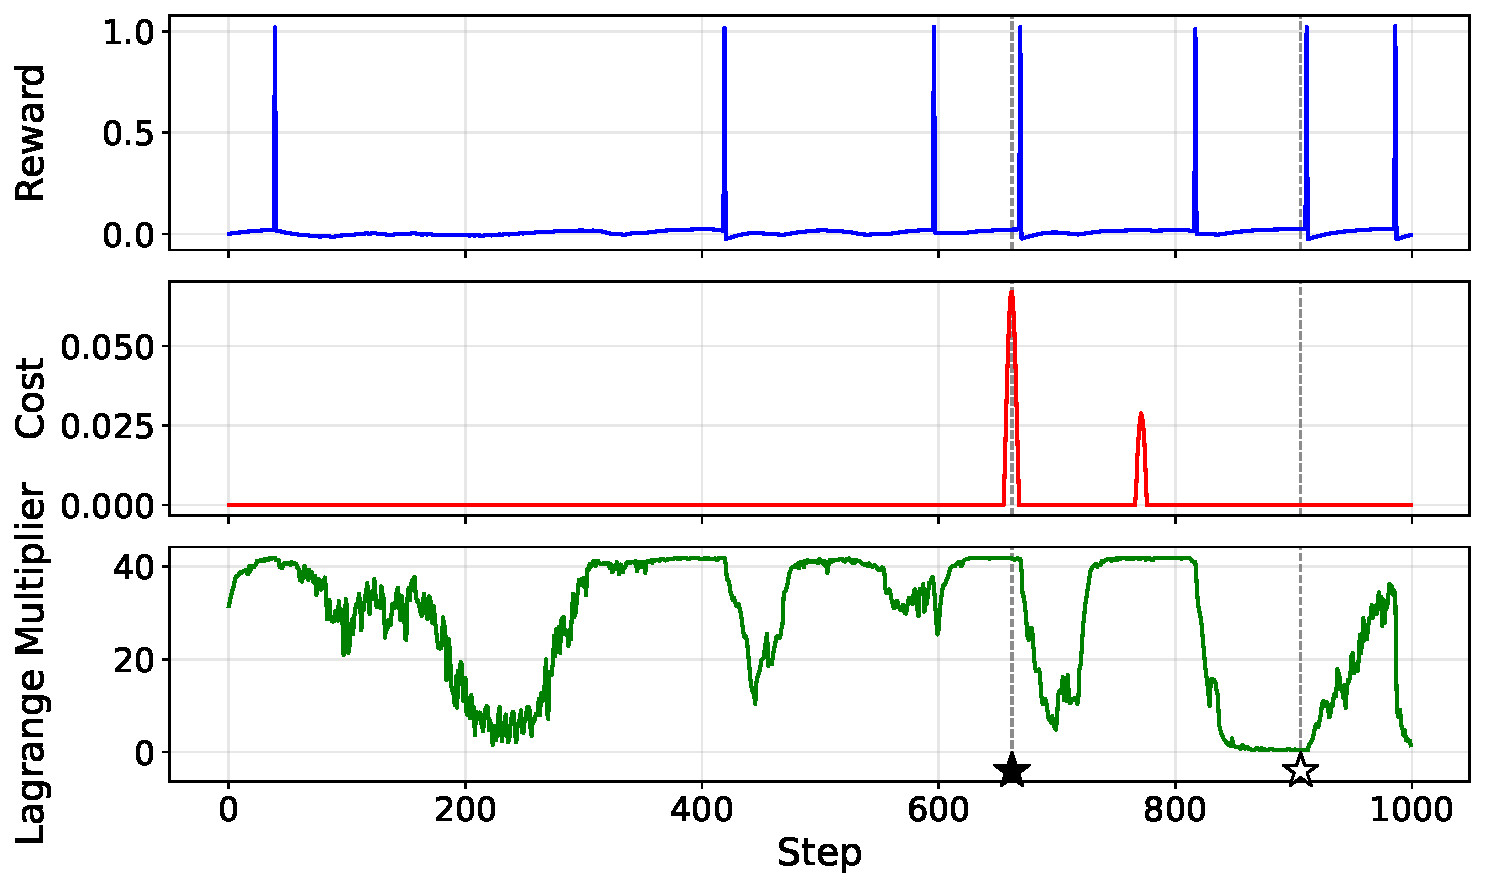
\includegraphics[width=0.8\textwidth]{figure/test/result.pdf}
    \caption{Evaluation results of a single episode.
            The plot shows the per-step reward, cost, and the output of the learned Lagrange multiplier network, which takes the state as input and produces a state-wise Lagrange multiplier.
            This multiplier output increases as the agent approaches obstacles and constraint violations, while it decreases toward zero when the agent remains in safe states.
            Frames at the timesteps marked with stars are shown in Fig.~\ref{fig:point_goal_test_results_bc}.}
    \label{fig:point_goal_test_results_a}
\end{figure}

\begin{figure}[H]
    \centering
    \begin{subfigure}{0.48\textwidth}
        \centering
        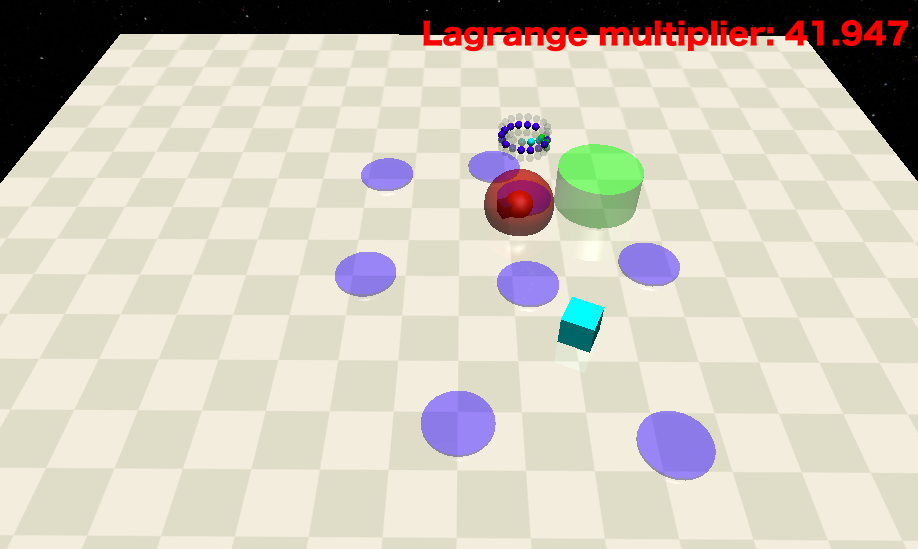
\includegraphics[width=\linewidth]{figure/test/unsafe.png}
        \caption{}
    \end{subfigure}
    \hfill
    \begin{subfigure}{0.49\textwidth}
        \centering
        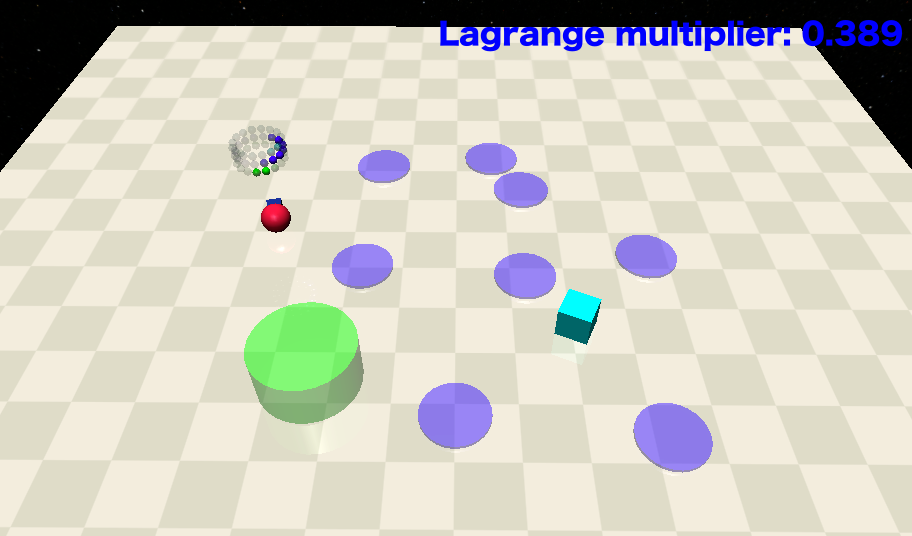
\includegraphics[width=\linewidth]{figure/test/safe.png}
        \caption{}
    \end{subfigure}
    \caption{%Frames from the same episode at the timesteps marked with stars in Fig. ~\ref{fig:point_goal_test_results_a}.  % 이 문장 삭제?
            Subfigure (a) shows the agent violating the constraint, where the network outputs its maximum value, 
            while subfigure (b) shows the agent in a safe situation, where the output remains close to zero.}
    \label{fig:point_goal_test_results_bc}
\end{figure}

Figures~\ref{fig:point_goal_test_results_a} and \ref{fig:point_goal_test_results_bc} present the evaluation results of the learned Lagrange multiplier network. 
The network takes the state as input and produces a state-wise Lagrange multiplier at each timestep.
Figure~\ref{fig:point_goal_test_results_a} shows the per-step reward, cost, and the output of the network throughout a single episode.
The output increases as the agent approaches obstacles and potential constraint violations, while decreasing toward zero when the agent remains in safe states, as observed from the green curve in the bottom subplot of Fig.~\ref{fig:point_goal_test_results_a}.
Figure~\ref{fig:point_goal_test_results_bc} shows simulation frames corresponding to the two starred timesteps in Fig.~\ref{fig:point_goal_test_results_a}: the black star corresponds to subfigure (a), where the agent violates the constraint and the multiplier reaches its maximum value, while the white star corresponds to subfigure (b), where the agent remains in a safe state and the output stays close to zero.